\documentclass{ximera}

%\usepackage{todonotes}

\newcommand{\todo}{}

\usepackage{esint} % for \oiint
\ifxake%%https://math.meta.stackexchange.com/questions/9973/how-do-you-render-a-closed-surface-double-integral
\renewcommand{\oiint}{{\large\bigcirc}\kern-1.56em\iint}
\fi


\graphicspath{
  {./}
  {ximeraTutorial/}
  {basicPhilosophy/}
  {functionsOfSeveralVariables/}
  {normalVectors/}
  {lagrangeMultipliers/}
  {vectorFields/}
  {greensTheorem/}
  {shapeOfThingsToCome/}
  {dotProducts/}
  {partialDerivativesAndTheGradientVector/}
  {../productAndQuotientRules/exercises/}
  {../normalVectors/exercisesParametricPlots/}
  {../continuityOfFunctionsOfSeveralVariables/exercises/}
  {../partialDerivativesAndTheGradientVector/exercises/}
  {../directionalDerivativeAndChainRule/exercises/}
  {../commonCoordinates/exercisesCylindricalCoordinates/}
  {../commonCoordinates/exercisesSphericalCoordinates/}
  {../greensTheorem/exercisesCurlAndLineIntegrals/}
  {../greensTheorem/exercisesDivergenceAndLineIntegrals/}
  {../shapeOfThingsToCome/exercisesDivergenceTheorem/}
  {../greensTheorem/}
  {../shapeOfThingsToCome/}
  {../separableDifferentialEquations/exercises/}
  {vectorFields/}
}

\newcommand{\mooculus}{\textsf{\textbf{MOOC}\textnormal{\textsf{ULUS}}}}

\usepackage{tkz-euclide}
\usepackage{tikz}
\usepackage{tikz-cd}
\usetikzlibrary{arrows}
\tikzset{>=stealth,commutative diagrams/.cd,
  arrow style=tikz,diagrams={>=stealth}} %% cool arrow head
\tikzset{shorten <>/.style={ shorten >=#1, shorten <=#1 } } %% allows shorter vectors

\usetikzlibrary{backgrounds} %% for boxes around graphs
\usetikzlibrary{shapes,positioning}  %% Clouds and stars
\usetikzlibrary{matrix} %% for matrix
\usepgfplotslibrary{polar} %% for polar plots
\usepgfplotslibrary{fillbetween} %% to shade area between curves in TikZ
%\usetkzobj{all}
\usepackage[makeroom]{cancel} %% for strike outs
%\usepackage{mathtools} %% for pretty underbrace % Breaks Ximera
%\usepackage{multicol}
\usepackage{pgffor} %% required for integral for loops



%% http://tex.stackexchange.com/questions/66490/drawing-a-tikz-arc-specifying-the-center
%% Draws beach ball
\tikzset{pics/carc/.style args={#1:#2:#3}{code={\draw[pic actions] (#1:#3) arc(#1:#2:#3);}}}



\usepackage{array}
\setlength{\extrarowheight}{+.1cm}
\newdimen\digitwidth
\settowidth\digitwidth{9}
\def\divrule#1#2{
\noalign{\moveright#1\digitwidth
\vbox{\hrule width#2\digitwidth}}}




% \newcommand{\RR}{\mathbb R}
% \newcommand{\R}{\mathbb R}
% \newcommand{\N}{\mathbb N}
% \newcommand{\Z}{\mathbb Z}

\newcommand{\sagemath}{\textsf{SageMath}}


%\renewcommand{\d}{\,d\!}
%\renewcommand{\d}{\mathop{}\!d}
%\newcommand{\dd}[2][]{\frac{\d #1}{\d #2}}
%\newcommand{\pp}[2][]{\frac{\partial #1}{\partial #2}}
% \renewcommand{\l}{\ell}
%\newcommand{\ddx}{\frac{d}{\d x}}

% \newcommand{\zeroOverZero}{\ensuremath{\boldsymbol{\tfrac{0}{0}}}}
%\newcommand{\inftyOverInfty}{\ensuremath{\boldsymbol{\tfrac{\infty}{\infty}}}}
%\newcommand{\zeroOverInfty}{\ensuremath{\boldsymbol{\tfrac{0}{\infty}}}}
%\newcommand{\zeroTimesInfty}{\ensuremath{\small\boldsymbol{0\cdot \infty}}}
%\newcommand{\inftyMinusInfty}{\ensuremath{\small\boldsymbol{\infty - \infty}}}
%\newcommand{\oneToInfty}{\ensuremath{\boldsymbol{1^\infty}}}
%\newcommand{\zeroToZero}{\ensuremath{\boldsymbol{0^0}}}
%\newcommand{\inftyToZero}{\ensuremath{\boldsymbol{\infty^0}}}



% \newcommand{\numOverZero}{\ensuremath{\boldsymbol{\tfrac{\#}{0}}}}
% \newcommand{\dfn}{\textbf}
% \newcommand{\unit}{\,\mathrm}
% \newcommand{\unit}{\mathop{}\!\mathrm}
% \newcommand{\eval}[1]{\bigg[ #1 \bigg]}
% \newcommand{\seq}[1]{\left( #1 \right)}
% \renewcommand{\epsilon}{\varepsilon}
% \renewcommand{\phi}{\varphi}


% \renewcommand{\iff}{\Leftrightarrow}

% \DeclareMathOperator{\arccot}{arccot}
% \DeclareMathOperator{\arcsec}{arcsec}
% \DeclareMathOperator{\arccsc}{arccsc}
% \DeclareMathOperator{\si}{Si}
% \DeclareMathOperator{\scal}{scal}
% \DeclareMathOperator{\sign}{sign}


%% \newcommand{\tightoverset}[2]{% for arrow vec
%%   \mathop{#2}\limits^{\vbox to -.5ex{\kern-0.75ex\hbox{$#1$}\vss}}}
% \newcommand{\arrowvec}[1]{{\overset{\rightharpoonup}{#1}}}
% \renewcommand{\vec}[1]{\arrowvec{\mathbf{#1}}}
% \renewcommand{\vec}[1]{{\overset{\boldsymbol{\rightharpoonup}}{\mathbf{#1}}}}

% \newcommand{\point}[1]{\left(#1\right)} %this allows \vector{ to be changed to \vector{ with a quick find and replace
% \newcommand{\pt}[1]{\mathbf{#1}} %this allows \vec{ to be changed to \vec{ with a quick find and replace
% \newcommand{\Lim}[2]{\lim_{\point{#1} \to \point{#2}}} %Bart, I changed this to point since I want to use it.  It runs through both of the exercise and exerciseE files in limits section, which is why it was in each document to start with.

% \DeclareMathOperator{\proj}{\mathbf{proj}}
% \newcommand{\veci}{{\boldsymbol{\hat{\imath}}}}
% \newcommand{\vecj}{{\boldsymbol{\hat{\jmath}}}}
% \newcommand{\veck}{{\boldsymbol{\hat{k}}}}
% \newcommand{\vecl}{\vec{\boldsymbol{\l}}}
% \newcommand{\uvec}[1]{\mathbf{\hat{#1}}}
% \newcommand{\utan}{\mathbf{\hat{t}}}
% \newcommand{\unormal}{\mathbf{\hat{n}}}
% \newcommand{\ubinormal}{\mathbf{\hat{b}}}

% \newcommand{\dotp}{\bullet}
% \newcommand{\cross}{\boldsymbol\times}
% \newcommand{\grad}{\boldsymbol\nabla}
% \newcommand{\divergence}{\grad\dotp}
% \newcommand{\curl}{\grad\cross}
%\DeclareMathOperator{\divergence}{divergence}
%\DeclareMathOperator{\curl}[1]{\grad\cross #1}
% \newcommand{\lto}{\mathop{\longrightarrow\,}\limits}

% \renewcommand{\bar}{\overline}

\colorlet{textColor}{black}
\colorlet{background}{white}
\colorlet{penColor}{blue!50!black} % Color of a curve in a plot
\colorlet{penColor2}{red!50!black}% Color of a curve in a plot
\colorlet{penColor3}{red!50!blue} % Color of a curve in a plot
\colorlet{penColor4}{green!50!black} % Color of a curve in a plot
\colorlet{penColor5}{orange!80!black} % Color of a curve in a plot
\colorlet{penColor6}{yellow!70!black} % Color of a curve in a plot
\colorlet{fill1}{penColor!20} % Color of fill in a plot
\colorlet{fill2}{penColor2!20} % Color of fill in a plot
\colorlet{fillp}{fill1} % Color of positive area
\colorlet{filln}{penColor2!20} % Color of negative area
\colorlet{fill3}{penColor3!20} % Fill
\colorlet{fill4}{penColor4!20} % Fill
\colorlet{fill5}{penColor5!20} % Fill
\colorlet{gridColor}{gray!50} % Color of grid in a plot

\newcommand{\surfaceColor}{violet}
\newcommand{\surfaceColorTwo}{redyellow}
\newcommand{\sliceColor}{greenyellow}




\pgfmathdeclarefunction{gauss}{2}{% gives gaussian
  \pgfmathparse{1/(#2*sqrt(2*pi))*exp(-((x-#1)^2)/(2*#2^2))}%
}


%%%%%%%%%%%%%
%% Vectors
%%%%%%%%%%%%%

%% Simple horiz vectors
\renewcommand{\vector}[1]{\left\langle #1\right\rangle}


%% %% Complex Horiz Vectors with angle brackets
%% \makeatletter
%% \renewcommand{\vector}[2][ , ]{\left\langle%
%%   \def\nextitem{\def\nextitem{#1}}%
%%   \@for \el:=#2\do{\nextitem\el}\right\rangle%
%% }
%% \makeatother

%% %% Vertical Vectors
%% \def\vector#1{\begin{bmatrix}\vecListA#1,,\end{bmatrix}}
%% \def\vecListA#1,{\if,#1,\else #1\cr \expandafter \vecListA \fi}

%%%%%%%%%%%%%
%% End of vectors
%%%%%%%%%%%%%

%\newcommand{\fullwidth}{}
%\newcommand{\normalwidth}{}



%% makes a snazzy t-chart for evaluating functions
%\newenvironment{tchart}{\rowcolors{2}{}{background!90!textColor}\array}{\endarray}

%%This is to help with formatting on future title pages.
\newenvironment{sectionOutcomes}{}{}



%% Flowchart stuff
%\tikzstyle{startstop} = [rectangle, rounded corners, minimum width=3cm, minimum height=1cm,text centered, draw=black]
%\tikzstyle{question} = [rectangle, minimum width=3cm, minimum height=1cm, text centered, draw=black]
%\tikzstyle{decision} = [trapezium, trapezium left angle=70, trapezium right angle=110, minimum width=3cm, minimum height=1cm, text centered, draw=black]
%\tikzstyle{question} = [rectangle, rounded corners, minimum width=3cm, minimum height=1cm,text centered, draw=black]
%\tikzstyle{process} = [rectangle, minimum width=3cm, minimum height=1cm, text centered, draw=black]
%\tikzstyle{decision} = [trapezium, trapezium left angle=70, trapezium right angle=110, minimum width=3cm, minimum height=1cm, text centered, draw=black]


\title{Theory}

\begin{document}

\begin{abstract}
the logarithmic story
\end{abstract}
\maketitle



$\log_A(B)$ is pronounced ``the logarithm base $A$ of $B$'' or ``the log base $A$ of $B$'' or ``the logarithm of $B$ base $A$''. \\




\begin{center}
\textbf{\textcolor{red!80!black}{$\log_A(B)$ is the thing you raise $A$ to, to get $B$.}} \\

\textbf{\textcolor{purple!85!blue}{this is the magic sentence}}
\end{center}


Logarithms are exponents.  They are the things we raise bases to, to get targeted outputs. Therefore, to understand logarithms, we should investigate the exponents in exponential functions. \\











An example of a basic exponential function is $E(t) = 2^t$.  

Its graph looks like







\begin{image}
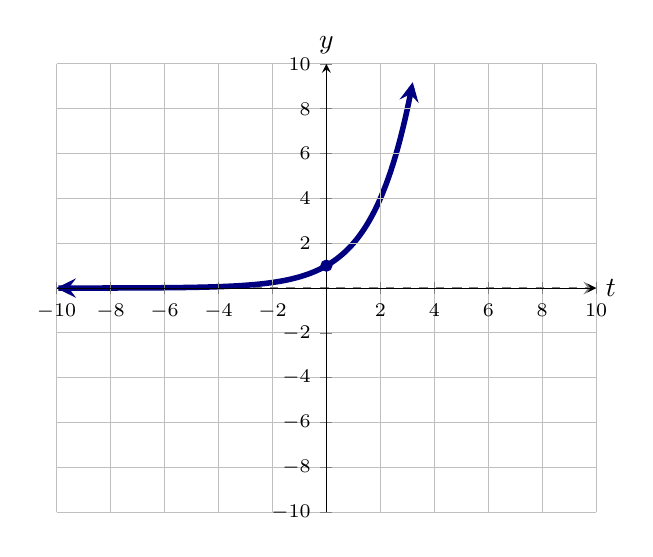
\begin{tikzpicture}
  \begin{axis}[
            domain=-10:10, ymax=10, xmax=10, ymin=-10, xmin=-10,
            axis lines =center, xlabel=$t$, ylabel=$y$, grid = major,
            ytick={-10,-8,-6,-4,-2,2,4,6,8,10},
          	xtick={-10,-8,-6,-4,-2,2,4,6,8,10},
          	ticklabel style={font=\scriptsize},
            every axis y label/.style={at=(current axis.above origin),anchor=south},
            every axis x label/.style={at=(current axis.right of origin),anchor=west},
            axis on top
          ]
          
          	\addplot [line width=1, gray, dashed,samples=200,domain=(-10:10),<->] {0};

      		\addplot [line width=2, penColor, smooth,samples=200,domain=(-10:3.2),<->] {2^x};

      		\addplot[color=penColor,fill=penColor,only marks,mark=*] coordinates{(0,1)};

          


  \end{axis}
\end{tikzpicture}
\end{image}

$E(t)$ is an increasing function, which means when we select a greater exponent in the domain, then we get a greater function value.  



We can see this by evaluating our exponential function with increasing domain numbers:
\begin{itemize}
\item $E(-1) = 2^{-1} = \frac{1}{2}$
\item $E(0) = 2^0 = 1$
\item $E\left(\frac{1}{2}\right) = 2^{\tfrac{1}{2}} = \sqrt{2}$
\end{itemize}


When we evaluate this exponential function, we know the domain number and we seek its range partner. In this case, we select $d$ from the domain and we assemble the pair $(d, 2^d)$, where $2^d$ is the value of the function, $E(t)$, at $d$.



Here we are supplying an exponent from the domain and then obtaining a function value for the exponential function.  We can look at this process in reverse: we select a function value and we are in search of an exponent that will produce the desired output.









\section*{Reverse}

How do we think about $E(t) = 2^t$ in reverse?
\begin{itemize}
\item $E(t) = {\tfrac{1}{4}} $
\item $E(t) = 4$
\item $E(t) = 16 $
\end{itemize}


Here, we know the desired value of the function.  We seek the domain numbers paired with it. We seek the exponent. We know $2^d$, we seek the pair $(d, 2^d)$, where $d$ is the solution to the equation $E(t) = 2^d$.




\textbf{\textcolor{red!90!darkgray}{$\bigstar$}}  Since $E(t) = 2^t > 0$ for any $t$, thinking backwards only works if we provide positive function values. $2^t$ cannot equal a negative value. $2^t$ cannot equal $0$.   \\ 



\textbf{\textcolor{red!90!darkgray}{$\bigstar$}} For $E(t) = 2^t$, every positive function value has \textit{exactly one} associated domain number, one exponent, one \textbf{\textcolor{purple!85!blue}{logarithm}}. (That is eeriely similar to the function rule for pairs in the exponential function.) \\ 




Thinking of an exponential function in reverse sounds like a new function. We call it a \textbf{\textcolor{purple!85!blue}{logarithmic function}}.   \\


\begin{itemize}
\item In reverse, the range of an exponential function becomes the domain of a logarithmic function.
\item In reverse, the domain of an exponential function becomes the range of a logarithmic function.
\end{itemize}





\[
\begin{array}{lcl}
\text{Exponential Function}  &     &  \text{Logarithmic Function}  \\
domain = (-\infty, \infty)  &  \   &  domain = (0, \infty)  \\
range = (0, \infty)  &    &  range = (-\infty, \infty)  \\
(a, r^a)    &    &   (r^a, a)
\end{array}
\]


The basic logarithmic function just reverses the pairs in the basic exponential function.  If $(a, 2^a)$ is a pair in the exponential function, then $(2^a, a)$ is a pair in the logarithmic function.


Therefore, the domains and ranges switch. \\






\subsection*{Logarithm}

It seems weird to write $(2^a, a)$, even though it is perfectly correct.  We are supplying values of an exponential function, which look like $2^a$ and then the value of the logarithmic function is the needed exponent.

Instead, we are used to writing the domain number by a letter, like $b$, and then the function value as a formula involving $b$. That's what we are used to.

We would prefer our pairs in the logarithm function to look like 

\[ (b, expression)  \]







Logarithmic functions come from the study of \textbf{logarithms}, which is the study of the exponents, just like we are talking about. This gets shortened to \textbf{log} for notational purposes.  \\



In our example here, we are working with the base $2$ exponential function, $E(t) = 2^t$. So, the reverse is called \textbf{the logarithm base $2$}.  We tack on a subscript $2$ to the log to remind us of the base.



\[   \log_2(b)     \]


With this new symbol, we can describe pairs in the logarithmic function and points on its graph like 


\[
(b, \log_2(b))
\]


$\log_2(b)$ is just the exponent that $2$ needs to equal $b$.





$\blacktriangleright$ \textbf{Remember:} These pairs, $(b, \log_2(b))$, are the reverse of the exponential pairs : $(a, 2^a)$.  Therefore, $(b, \log_2(b))$ is also $(2^c, c)$ for some $c$. \\

$\blacktriangleright$  $\log_2(b)$ is the exponent, so that $2^? = b$ \\


$\blacktriangleright$  $\log_2(b)$ is the number that you raise $2$ to, to get $b$.  \\

\[   2^{\log_2(b)} = b     \]

We have a logarithmic function for every exponential function.  They are designated by their bases.














\begin{definition} \textbf{\textcolor{green!50!black}{Logarithm Base $r$ Function : $\log_r(x)$}}


$\log_r(x)$ is the number you raise $r$ to, to get $x$. \\

The domain is $(0, \infty)$. \\

The range is $(-\infty, \infty)$.


\end{definition}




\begin{conclusion}

\begin{itemize}
\item $\log_A(1)$ is the thing you raise $A$ to, to get $1$. Therefore, $\log_A(1) = 0$, since $A^0 = 1$
\item $\log_A(A)$ is the thing you raise $A$ to, to get $A$. Therefore, $\log_A(A) = 1$, since $A^1 = A$
\item $\log_A(\tfrac{1}{A})$ is the thing you raise $A$ to, to get $\tfrac{1}{A}$. Therefore, $\log_A(\tfrac{1}{A}) = -1$, since $A^{-1} = \tfrac{1}{A}$
\item $\log_A(A^n)$ is the thing you raise $A$ to, to get $A^n$. Therefore, $\log_A(A^n) = n$, since $A^n = A^n$
\end{itemize}

\end{conclusion}





\subsection*{Graphs}

Since all of the pairs of exponential and logarithmic functions are reversed, the graphs switch axes.



The horizontal axis is an asymptote for the graph of a basic exponential function. Switching axes makes the vertical axis an asymptote for the graph of a basic logarithmic function.


The graph of a basic exponential function has $(0,1)$ as an intercept.  The graph of a basic logarithmic function has $(1,0)$ as an intercept. 


Their graphs are mirror images of each other across the diagonal through quandrants I and III.










\begin{image}
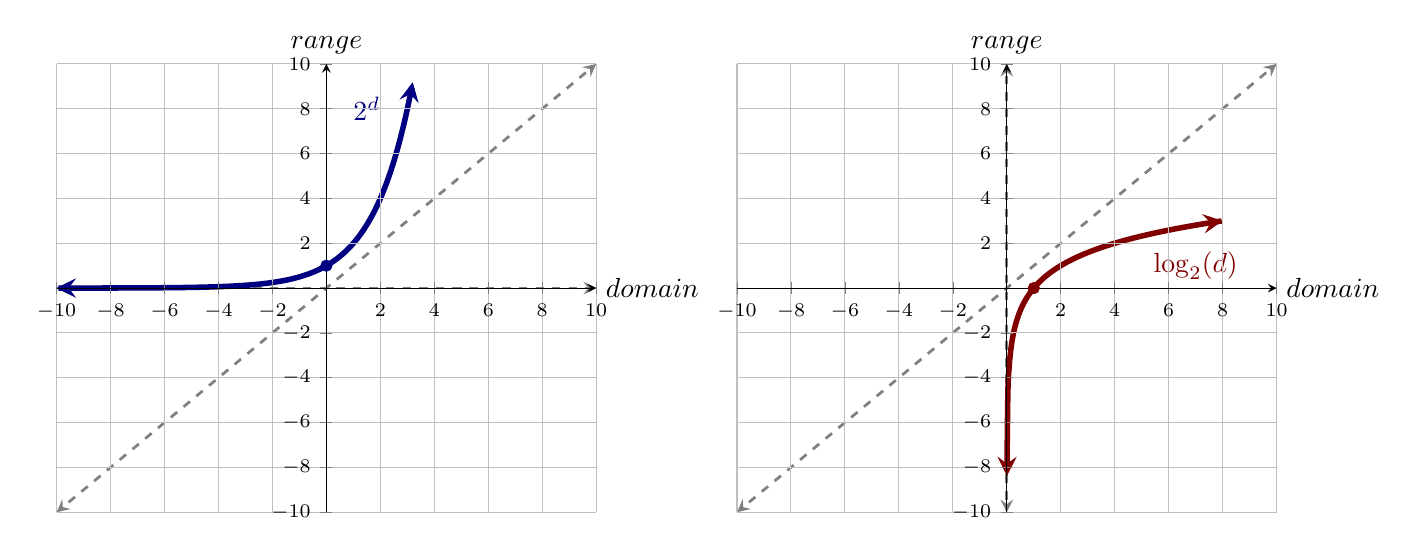
\begin{tikzpicture}



  \begin{axis}[name=invexp,
            domain=-10:10, ymax=10, xmax=10, ymin=-10, xmin=-10,
            axis lines =center, xlabel=$domain$, ylabel=$range$, grid = major,
            ytick={-10,-8,-6,-4,-2,2,4,6,8,10},
          	xtick={-10,-8,-6,-4,-2,2,4,6,8,10},
          	ticklabel style={font=\scriptsize},
            every axis y label/.style={at=(current axis.above origin),anchor=south},
            every axis x label/.style={at=(current axis.right of origin),anchor=west},
            axis on top
          ]
          
          	\addplot [line width=1, gray, dashed,samples=200,domain=(-10:10),<->] {0};

          	\addplot [line width=1, gray, dashed,samples=200,domain=(-10:10),<->] ({x},{x});

      		\addplot [line width=2, penColor, smooth,samples=200,domain=(-10:3.2),<->] {2^x};


          	


      		\addplot[color=penColor,fill=penColor,only marks,mark=*] coordinates{(0,1)};


      		\node[penColor] at (axis cs:1.5,8) {$2^d$};

  \end{axis}
  \begin{axis}[at={(invexp.outer east)},anchor=outer west,
            domain=-10:10, ymax=10, xmax=10, ymin=-10, xmin=-10,
            axis lines =center, xlabel=$domain$, ylabel=$range$, grid = major,
            ytick={-10,-8,-6,-4,-2,2,4,6,8,10},
            xtick={-10,-8,-6,-4,-2,2,4,6,8,10},
            ticklabel style={font=\scriptsize},
            every axis y label/.style={at=(current axis.above origin),anchor=south},
            every axis x label/.style={at=(current axis.right of origin),anchor=west},
            axis on top
          ]
          

            \addplot [line width=1, gray, dashed,samples=200,domain=(-10:10),<->] ({0},{x});
            \addplot [line width=1, gray, dashed,samples=200,domain=(-10:10),<->] ({x},{x});


          \addplot [line width=2, penColor2, smooth,samples=200,domain=(0.003:8),<->] {ln(x)/ln(2)};

            


          \addplot[color=penColor2,fill=penColor2,only marks,mark=*] coordinates{(1,0)};

          \node[penColor2] at (axis cs:7,1) {$\log_2(d)$};
    \end{axis}




\end{tikzpicture}
\end{image}




From this basic logarithmic function and its graph we can transform and analyze more general logarithmic functions.







\begin{fact}


Logarithmic functions don't really have vertically shifted versions.  We can talk about a basic logarithm function being shifted.

\[
L(x) = A \log_r(B \, x + C) + D
\]


But, the $D$ can be explained with additional horizontal transformations, like this... \\


\begin{explanation}

We know that the range of $\log_r(x)$ is all real numbers, which includes $D$.  Therefore, there must be a real number, $d$, such that $\log_r(d) = D$. \\


That gives us 



\[
L(x) = A \log_r(B \, x + C) + D = A \log_r(B \, x + C) + \log_r(d)
\]

And, we have logarithm rules, which give us


\[
L(x) = A \log_r(B \, x + C) + D = A \log_r((B \, x + C)d) = A \log_r(B \, d \, x + C \, d) 
\]

\end{explanation}

Therefore, we separate exponential and shifted exponential, but we don't separate logarithmic and shifted logarithmic.

\end{fact}


\textbf{Note:}  Many times people just speak about exponential functions, and they mean both exponential and shifted exponential.




























\begin{example}  



Analyze   $M(t) = \log_2(t+3) - 4$ \\



We'll begin by thinking about the graph to help our analysis. \\


\begin{idea}


$\blacktriangleright$ First, the base is $2$, which is greater than $1$.

$\blacktriangleright$ The inside of the logarithm is $t+3$ and this equals $0$ when $t=-3$.  This must be the vertical asymptote.

$\blacktriangleright$ The inside of the logarithm is $t+3$, and this is positive for $t>-3$.  The graph must be on the right side of the vertical asymptote.

$\blacktriangleright$ The leading coefficient of $M$ is $1$, which is positive.  Therefore, the graph hugs the asymptote down the asymptote. 

$\blacktriangleright$ $t+3=1$ when $t=-2$. Therefore, the anchor point $(1,0)$ has moved to $t = -2$.  $M(-2) = -4$.  This gives us the point $(-2, -4)$.





Graph of $y = M(t)$.

\begin{image}
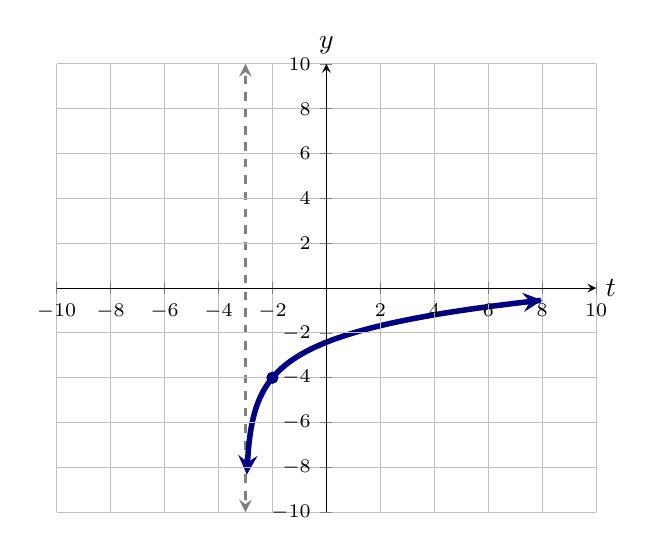
\begin{tikzpicture}
  \begin{axis}[
            domain=-10:10, ymax=10, xmax=10, ymin=-10, xmin=-10,
            axis lines =center, xlabel=$t$, ylabel=$y$, grid = major,
            ytick={-10,-8,-6,-4,-2,2,4,6,8,10},
            xtick={-10,-8,-6,-4,-2,2,4,6,8,10},
            ticklabel style={font=\scriptsize},
            every axis y label/.style={at=(current axis.above origin),anchor=south},
            every axis x label/.style={at=(current axis.right of origin),anchor=west},
            axis on top
          ]
          
			\addplot [line width=1, gray, dashed,samples=200,domain=(-10:10),<->] ({-3},{x});
			\addplot [line width=2, penColor, smooth,samples=200,domain=(-2.95:8),<->] {ln(x+3)/ln(2)-4};


			\addplot[color=penColor,fill=penColor,only marks,mark=*] coordinates{(-2,-4)};



  \end{axis}
\end{tikzpicture}
\end{image}


With these ideas, we can write an algebraic analysis. \\


\end{idea}






Now, for our function analysis.





\textbf{Domain}  

The inside of the logarithm is positive on $(-3, \infty)$.  Therefore, the domain of $M$ is $(-3, \infty)$. \\


\textbf{Zeros}  

All logarithmic functions have a single zero. We see that this graph will have a horizontal intercept around $(11, 0)$.  \\


$M(t) = \log_2(t+3) - 4 = 0$ \\


\begin{align*}
\log_2(t+3) - 4 & = 0 \\
\log_2(t+3) & = 4 \\
2^{\log_2(t+3)} & = \answer{2^4} \\
\answer{t+3} & = 16 \\
t & = 13
\end{align*}


$\blacktriangleright$ \textbf{Remember:} $\log_2(t+3)$ is the thing that you raise $2$ to, to get $t+3$ and $\log_2(t+3) = 4$.  Therefore, $4$ is also the thing that you raise $2$ to, to get $t+3$. Therefore, $t+3$ must be $16$.




\textbf{Continuity}  


Logarithmic functions are continuous.  That is a property of all logarithmic functions. \\


\textbf{End-Behavior} 

We are comparing back to our choice for a basic basic logarithmic function.  If we chose $\ln(x)$, then we can inventory the pieces of the formula for $M$ and compare back to $\ln(x)$, which is an increasing function.  \\



The base of $M$ is $2 > 1$, so this does not change the behavior.
The leading coefficient of $M$ is $1$, which is positive, so this does not change the behavior. 
the leading coefficient of the linear inside is $1$, which is also positive, so this does not change the behavior.

$M$ is an increasing function. \\  








\textbf{End-Behavior} 

$M$ is an increasing function on $(-3, \infty)$.\\

\[
\lim\limits_{t \to -3^+} M(t) = -\infty
\]

\[
\lim\limits_{t \to \infty} M(t) = \infty
\]





\textbf{Global Extrema} 

Logarithmic functions do not have global maximums or minimums. \\


\textbf{Local Extrema:} 

Logarithmic functions do not have local maximums or minimums. \\



\textbf{Range:} 

The range of every logarithmic function is $(-\infty, \infty)$.






\end{example}

























In this example, $M(t)$ is a logarithmic function, so it must have an inverse partner exponential function.  The pairs for $M$ look like $(t, M(t))$ or just $(t,M)$. The pairs for the exponential function would look like $(M, t)$.  The roles of $M$ and $t$ would be switched. $M$ would be the variable in the formula. $t$ would be the function value.\\


$M = \log_2(t+3) - 4$ is an equation describing both the logarithmic function, $M(t)$, and the exponential function $t(M)$.  We just are used to having the function name by itself on one side of the equal sign. \\


We can obtain such a formula for this partner exponential function by solving the logarithmic equation for $t$.





\begin{align*}
\log_2(t+3) - 4 & = M \\
\log_2(t+3) & = M + 4 \\
2^{\log_2(t+3)} & = 2^{M+4} \\
t+3 & = 2^{M+4} \\
t & = 2^{M+4} - 3
\end{align*}


$\blacktriangleright$ \textbf{Remember:} $\log_2(t+3)$ is the thing that you raise $2$ to, to get $t+3$ and $\log_2(t+3) = M+4$.  Therefore, $M+4$ is the thing that you raise $2$ to, to get $t+3$





Here is the graph of both the logarithmic and the associated exponential functions. They are inverses of each other.





\begin{image}
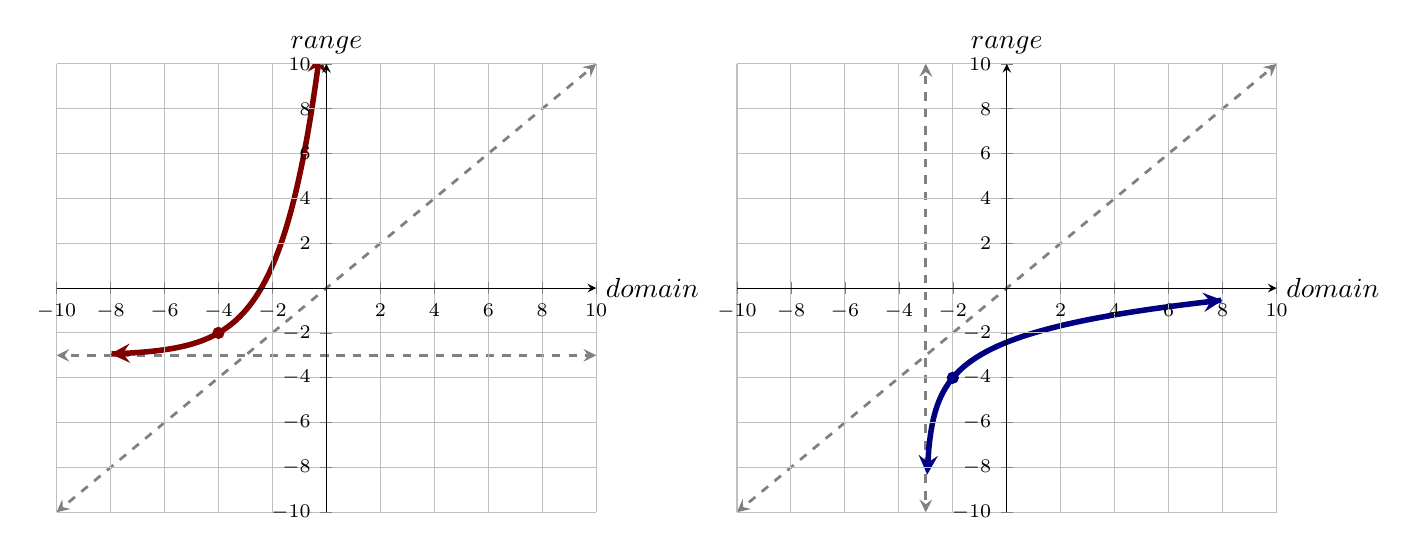
\begin{tikzpicture}

  \begin{axis}[name=invexp2,
            domain=-10:10, ymax=10, xmax=10, ymin=-10, xmin=-10,
            axis lines =center, xlabel=$domain$, ylabel=$range$, grid = major,
            ytick={-10,-8,-6,-4,-2,2,4,6,8,10},
            xtick={-10,-8,-6,-4,-2,2,4,6,8,10},
            ticklabel style={font=\scriptsize},
            every axis y label/.style={at=(current axis.above origin),anchor=south},
            every axis x label/.style={at=(current axis.right of origin),anchor=west},
            axis on top
          ]
          

            \addplot [line width=1, gray, dashed,samples=200,domain=(-10:10),<->] ({x},{-3});
            \addplot [line width=1, gray, dashed,samples=200,domain=(-10:10),<->] ({x},{x});


			\addplot [line width=2, penColor2, smooth,samples=200,domain=(-8:-0.25),<->] {2^(x+4)-3};



			\addplot[color=penColor2,fill=penColor2,only marks,mark=*] coordinates{(-4,-2)};
  \end{axis}
  \begin{axis}[at={(invexp2.outer east)},anchor=outer west,
            domain=-10:10, ymax=10, xmax=10, ymin=-10, xmin=-10,
            axis lines =center, xlabel=$domain$, ylabel=$range$, grid = major,
            ytick={-10,-8,-6,-4,-2,2,4,6,8,10},
            xtick={-10,-8,-6,-4,-2,2,4,6,8,10},
            ticklabel style={font=\scriptsize},
            every axis y label/.style={at=(current axis.above origin),anchor=south},
            every axis x label/.style={at=(current axis.right of origin),anchor=west},
            axis on top
          ]
          
      \addplot [line width=1, gray, dashed,samples=200,domain=(-10:10),<->] ({-3},{x});

            \addplot [line width=1, gray, dashed,samples=200,domain=(-10:10),<->] ({x},{x});

      \addplot [line width=2, penColor, smooth,samples=200,domain=(-2.95:8),<->] {ln(x+3)/ln(2)-4};



      \addplot[color=penColor,fill=penColor,only marks,mark=*] coordinates{(-2,-4)};

  \end{axis}


\end{tikzpicture}
\end{image}

































\begin{example}  


Analyze   $K(x) = -2 \, \log_3(4-x)$ \\



Categorize: $K(x) = -2 \, \log_3(4-x)$ is a logarithmic function, because it matches out template, $A \, \log_r(B \, x + C) + D$. \\


We'll begin by thinking about the graph to help guide our analysis. \\

\begin{idea}


$\blacktriangleright$ First, the base is $3$, which is greater than $1$.

$\blacktriangleright$ The inside of the logarithm is $4-x$, and this equals $0$ when $x=4$.  Therefore, $x=4$ has to be the vertical asymptote.

$\blacktriangleright$ The inside of the logarithm is $4-x$, and this is positive for $x<4$.  The graph must be on the left side of the vertical asymptote.

$\blacktriangleright$ The leading coefficient is $-2$, which is negative.  Therefore, the graph is flipped \wordChoice{\choice[correct]{vertically} \choice{horizontally}} from the basic graph. It goes up the asymptote. 

$\blacktriangleright$ $4-x=1$ when $x=3$. Therefore, the anchor point $(1,0)$ has moved to $\left( \answer{3}, 0 \right)$.





Graph of $y = K(x)$.

\begin{image}
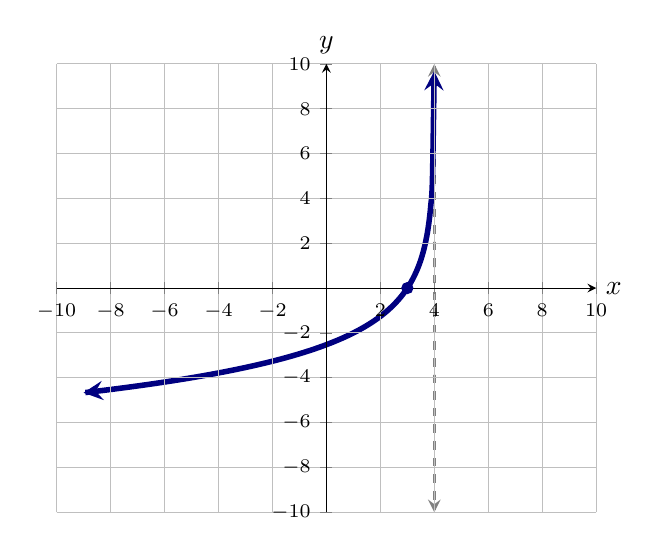
\begin{tikzpicture}
  \begin{axis}[
            domain=-10:10, ymax=10, xmax=10, ymin=-10, xmin=-10,
            axis lines =center, xlabel=$x$, ylabel=$y$, grid = major,
            ytick={-10,-8,-6,-4,-2,2,4,6,8,10},
            xtick={-10,-8,-6,-4,-2,2,4,6,8,10},
            ticklabel style={font=\scriptsize},
            every axis y label/.style={at=(current axis.above origin),anchor=south},
            every axis x label/.style={at=(current axis.right of origin),anchor=west},
            axis on top
          ]
          
      \addplot [line width=1, gray, dashed,samples=200,domain=(-10:10),<->] ({4},{x});
			\addplot [line width=2, penColor, smooth,samples=200,domain=(-9:3.995),<->] {-2*ln(4-x)/ln(3)};
      

		
            %\addplot [line width=1, gray, dashed,samples=200,domain=(-10:10),<->] ({x},{x});


			\addplot[color=penColor,fill=penColor,only marks,mark=*] coordinates{(3,0)};






           

  \end{axis}
\end{tikzpicture}
\end{image}



With these ideas, we can write an algebraic analysis. \\


\end{idea}





Now, for our function analysis.





\textbf{Domain}  

The inside of the logarithm is positive on $(-\infty, 4)$.  Therefore, the domain of $K$ is $(-\infty, 4)$. \\


\textbf{Zeros}  

We see that the graph is suggesting that the zero is around $3$. \\


$K(x) = -2 \, \log_3(4 - x) = 0$ \\


\begin{align*}
-2 \, \log_3(4 - x) & = 0 \\
\log_2(4 - x) & = 0 \\
4 - x & = 1 \\
3 & = x 
\end{align*}


$\blacktriangleright$ \textbf{Remember} $\log_3(4 - x)$ is the thing that you raise $3$ to, to get $4 - x$ and $\log_3(4 - x) = 0$.  Since, $0$ is also the thing that you raise $3$ to, to get $4 - x$, we must have $4 - x$ must be $1$.




\textbf{Continuity}  

Logarithmic functions are continuous.  That is a property of all logarithmic functions. \\









\textbf{Behavior} 

We are comparing back to our choice for a basic basic logarithmic function.  If we chose $\ln(x)$, then we can inventory the pieces of the formula for $K$ and compare back to $\ln(x)$, which is an increasing function.  \\



The base of $K$ is $3 > 1$, so this does not change the behavior.
The leading coefficient of $K$ is $-2 < 0$ and this does change the behavior to decreasing. 
the leading coefficient of the linear inside is $-1$, which is also negative, so this again changes the behavior back to increasing.

$K$ is an increasing function. \\  







\textbf{End-Behavior} 

$K$ is an increasing function. on the domain $(-\infty, 4)$. That tell sus that 


\[
\lim\limits_{x \to -\infty} K(x) = -\infty
\]



\[
\lim\limits_{t \to 4^-} K(x) = \infty
\]





\textbf{Global Extrema} 

Logarithmic function do not have global maximums or minimums. \\


\textbf{Local Extrema} 

Logarithmic function do not have local maximums or minimums. \\



\textbf{Range} 

The range of every logarithmic function is $(-\infty, \infty)$.









\end{example}









Reversing all of the pairs will give the inverse exponential function.  \\



$K(x)$ is a logarithmic function, so it must have a partner exponential function.  The pairs for $K$ look like $(x, K)$. The pairs for the exponential function would look like $(K, x)$.  The roles of $K$ and $x$ would be switched. $K$ would be the variable in the exponential formula. $x$ would be the exponential function value.  $K$ would be the independent variable and $x$ would be the dependent variable.


We can obtain a nice formula for this partner exponential function by solving the logarithmic equation for $x$.





\begin{align*}
-2 \, \log_3(4-x) & = M \\
\log_3(4-x) & = -\frac{M}{2} \\
3^{\log_3(4-x)} & = 3^{-\frac{M}{2}} \\
4 - x & = 3^{-\frac{M}{2}} \\
4 - 3^{-\frac{M}{2}} & = x \\
\end{align*}




$\blacktriangleright$ \textbf{Remember:} $\log_3(4-x)$ is the thing that you raise $3$ to, to get $4-x$ and $\log_3(4-x) = - \frac{M}{2}$.  Therefore, $- \frac{M}{2}$ is the thing that you raise $3$ to, to get $4-x$.





Here is the graph of both the logarithmic and exponential functions.  They are reflected about the diagonal, because the functions are inverses of each other. 





\begin{image}
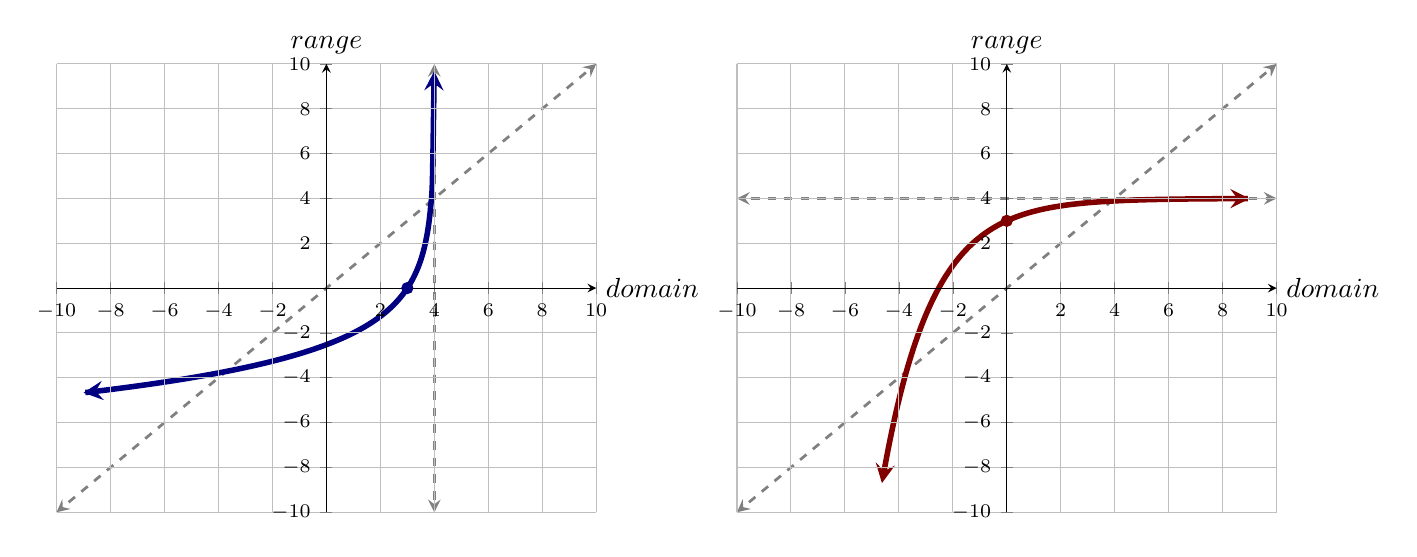
\begin{tikzpicture}

  \begin{axis}[name=invexp3,
            domain=-10:10, ymax=10, xmax=10, ymin=-10, xmin=-10,
            axis lines =center, xlabel=$domain$, ylabel=$range$, grid = major,
            ytick={-10,-8,-6,-4,-2,2,4,6,8,10},
            xtick={-10,-8,-6,-4,-2,2,4,6,8,10},
            ticklabel style={font=\scriptsize},
            every axis y label/.style={at=(current axis.above origin),anchor=south},
            every axis x label/.style={at=(current axis.right of origin),anchor=west},
            axis on top
          ]
          

          	\addplot [line width=1, gray, dashed,samples=200,domain=(-10:10),<->] ({4},{x});
          	\addplot [line width=1, gray, dashed,samples=200,domain=(-10:10),<->] ({x},{x});


			      \addplot [line width=2, penColor, smooth,samples=200,domain=(-9:3.995),<->] {-2*ln(4-x)/ln(3)};

			      \addplot[color=penColor,fill=penColor,only marks,mark=*] coordinates{(3,0)};


  \end{axis}
  \begin{axis}[at={(invexp3.outer east)},anchor=outer west,
            domain=-10:10, ymax=10, xmax=10, ymin=-10, xmin=-10,
            axis lines =center, xlabel=$domain$, ylabel=$range$, grid = major,
            ytick={-10,-8,-6,-4,-2,2,4,6,8,10},
            xtick={-10,-8,-6,-4,-2,2,4,6,8,10},
            ticklabel style={font=\scriptsize},
            every axis y label/.style={at=(current axis.above origin),anchor=south},
            every axis x label/.style={at=(current axis.right of origin),anchor=west},
            axis on top
          ]
          
            \addplot [line width=1, gray, dashed,samples=200,domain=(-10:10),<->] ({x},{4});

            \addplot [line width=1, gray, dashed,samples=200,domain=(-10:10),<->] ({x},{x});


            \addplot [line width=2, penColor2, smooth,samples=200,domain=(-4.627:9),<->] {4-3^(-x/2)};

            \addplot[color=penColor2,fill=penColor2,only marks,mark=*] coordinates{(0,3)};

  \end{axis}

\end{tikzpicture}
\end{image}








\begin{definition} \textbf{\textcolor{green!50!black}{Natural Logarithm}}   \\


The \textbf{natural logarithm} is the logarithm base $e$.  \\

It has special notation.

\[
\log_e(x) = \ln(x)
\]


$\ln(x)$ is the thing you raise $e$ to, to get $x$. \\


\textbf{Note:}  That is a lowercase ``el'' and a lowercase ``en''. It is not ``In''. 


\end{definition}



\begin{question}


Evaluate the following.

\begin{itemize}
\item $e^{\ln(4)} = \answer{4}$ 
\item $\ln(e^7) = \answer{7}$
\item $\ln\left( \frac{1}{e} \right) = \answer{-1}$
\end{itemize}



\end{question}



\begin{remark} \textbf{\textcolor{purple!85!blue}{e}} \\

\textbf{\textcolor{blue!55!black}{Remember:}} The function $\left( 1 + \frac{1}{x}  \right)^{x}$ has a limiting value.  Its end-behavior is a constant.  Its graph has a horizontal asymptote.  $e$ is this limiting value.

It might seem strange to select that number as the base for a logarithm and give it special notation.  However, it turns out that exponential functions with this base, $e$, are intricately connected to natural growth in the universe.

It is used A LOT!
\end{remark}










\begin{center}
\textbf{\textcolor{green!50!black}{ooooo-=-=-=-ooOoo-=-=-=-ooooo}} \\

more examples can be found by following this link\\ \link[More Examples of Logarithmic Functions]{https://ximera.osu.edu/csccmathematics/precalculus2/precalculus2/logFunctions/examples/exampleList}

\end{center}






\end{document}
